% !TEX root =  ../master.tex
\chapter{Nutzerhandbuch}\label{cha:Nutzerhandbuch}

Startet ein Nutzer die Anwendung, so wird er zu Beginn nach einem Token gefragt. Dieser Token ist der für die Kommunikation mit der Börse benötigte API Token und gewährleistet, dass mit der Börse nur Autorisierte Nutzer interagieren können. In unserer Anwendung wurde auf ein Login verzichtet, da bereits durch die Eingabe des API-Tokens gewährleistet wird, dass nur berechtigte Personen Simulationen starten können. 
\begin{figure}[ht]
	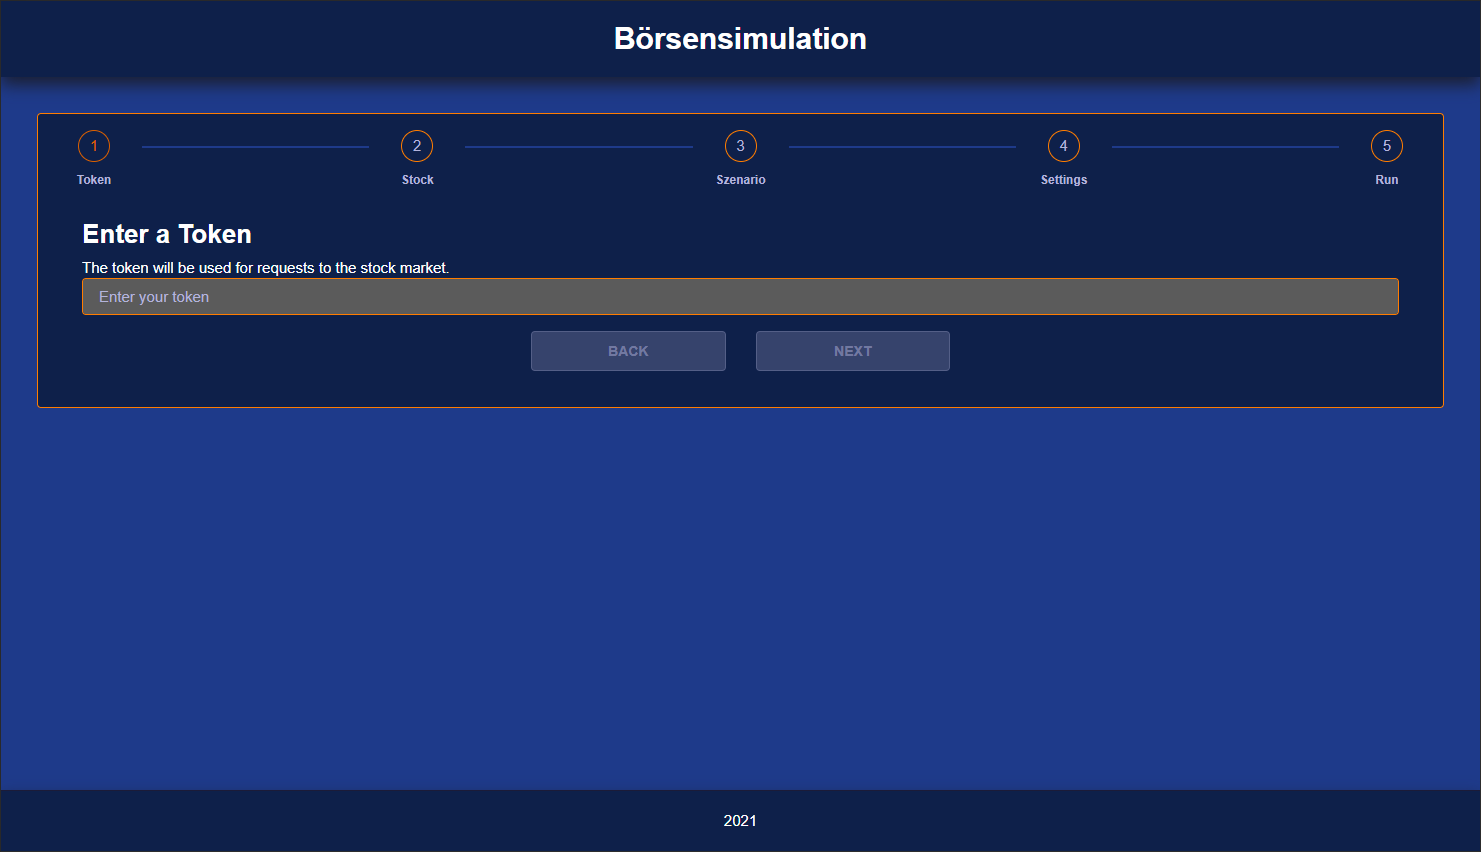
\includegraphics[width=\textwidth]{img/Token.png}
	\centering
	\caption{Start der Anwendung}
	\label{fig:token}
\end{figure}

Das überspringen dieses Schrittes ist wie in der Abbildung ersichtlich nicht möglich, da der Button next erst aktiviert wird, wenn ein Token eingegeben wurde. Dies wird aus Abbildung 6.1 und Abbildung 6.2 ersichtlich. Zudem bietet das gewählte Verfahren den Vorteil, dass der API Token nirgends in der Simulation gespeichert werden muss. So kann dieser auch nicht durch dritte ausgelesen werden oder muss im Rahmen eines ggf. vorhandenen Lifecycle Management des API-Managementsystems der Börse nicht im Code ausgetauscht werden. 
\begin{figure}[ht]
	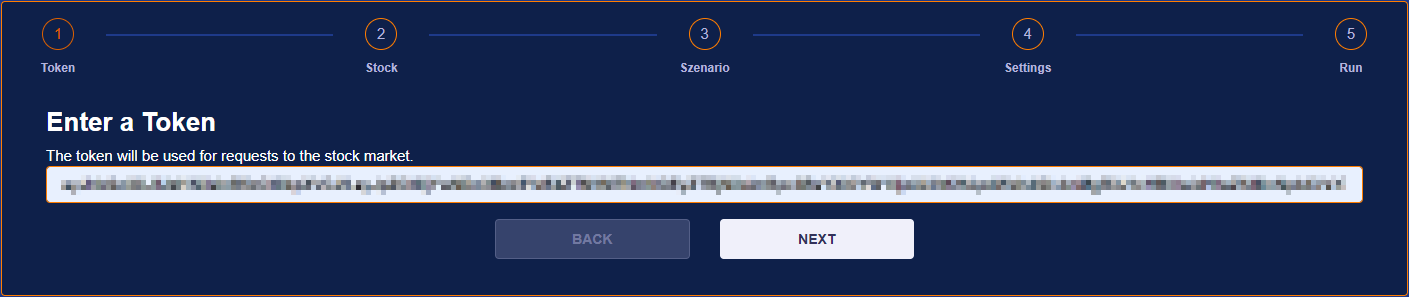
\includegraphics[width=\textwidth]{img/TokenInput.png}
	\centering
	\caption{Eingabe eines Tokens}
	\label{fig:tokeninput}
\end{figure}

Im nächsten Schritt, wählt der Nutzer eines der zur Verfügung stehenden Wertpapiere aus, für das er eine Simulation starten möchte. Hier stehen alle Wertpapiere zur Auswahl. Nimmt die Börse weitere Wertpapiere in den Handel auf, so werden diese auch sofort in dieser Liste aufgenommen.
\begin{figure}[ht]
	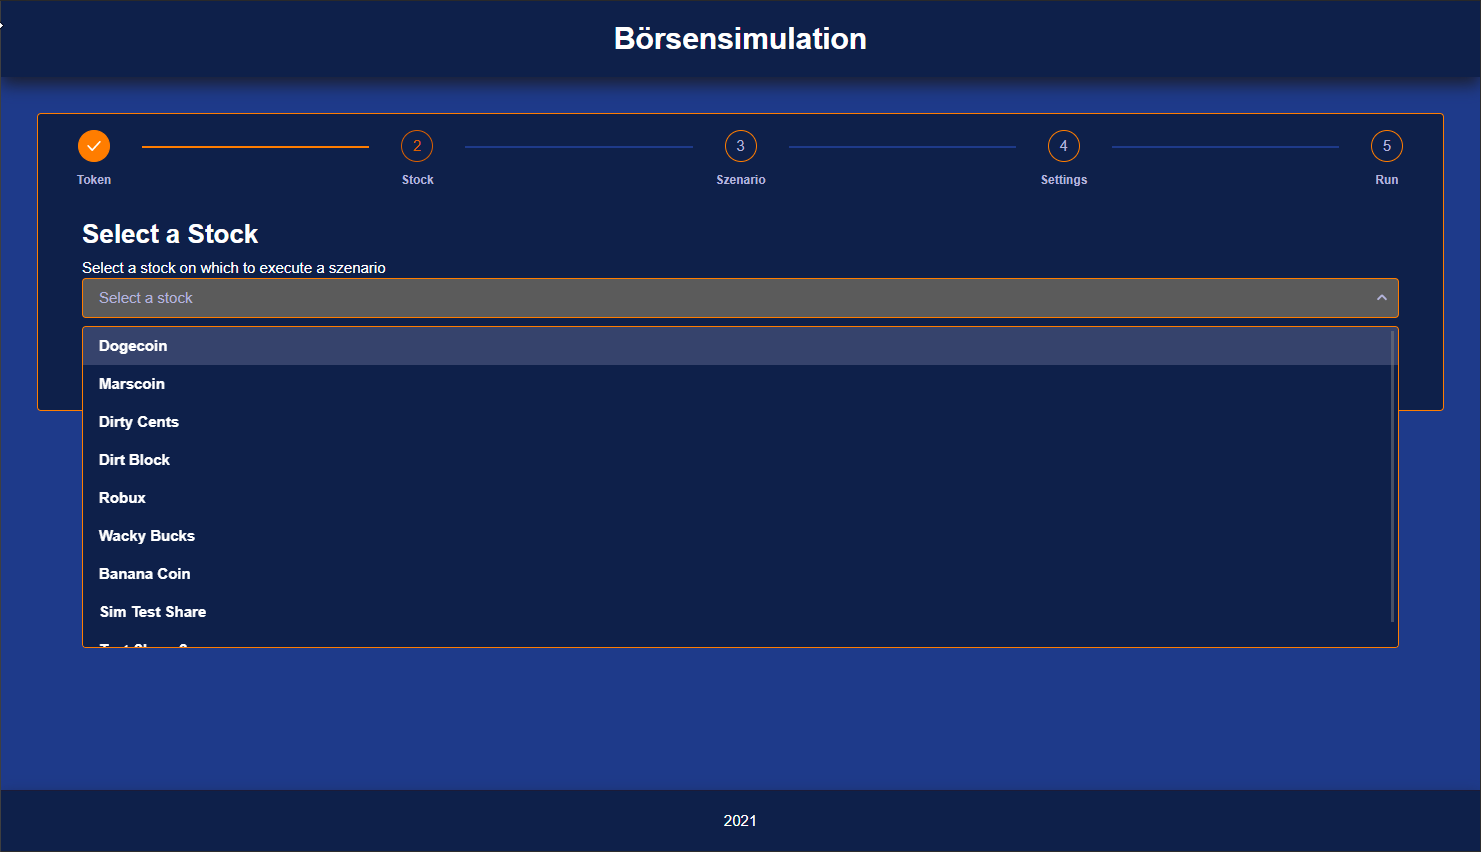
\includegraphics[width=\textwidth]{img/Stock.png}
	\centering
	\caption{Auswahl eines Wertpapiers}
	\label{fig:stock}
\end{figure}

Mit dem bestätigen des Next Buttons, gelangt der Nutzer zur Auswahl der Szenarien. Aktuell stehen dabei folgende Szenarien zur Verfügung:

\begin{itemize}
	\item Normaler Handelstag
	\item Positive Nachricht
	\item Geringes gehandeltes Volumen
	\item Kursabsturz durch Übernahme
	\item Hohes gehandeltes Volumen
\end{itemize}

Bei der Auswahl eines dieser Szenarien, wird darunter das simulierte Marktgeschehen dieses Szenarios angezeigt. Die Preise werden dabei als Delta aufgelistet, damit sie sich an die Kurswerte der einzelnen Wertpapiere anpassen und nicht die Preise auf ein gleiches Niveau drücken. Anschließend muss auch hier mit nächste bestätigt oder mit back in die zur Auswahl eines Wertpapieres zurückgekehrt werden. 
\begin{figure}[ht]
	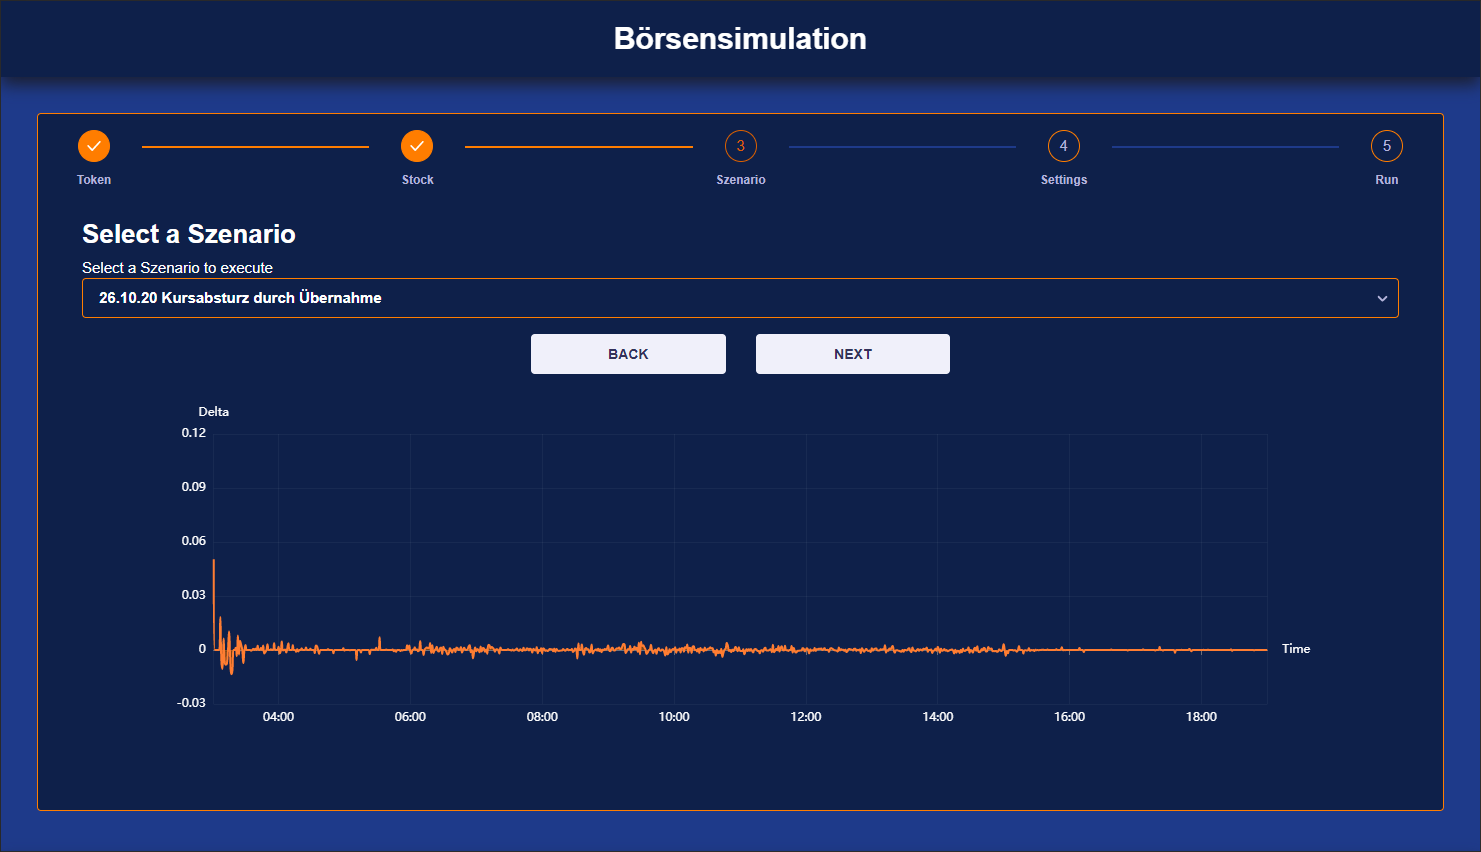
\includegraphics[width=\textwidth]{img/Szenario.png}
	\centering
	\caption{Auswahl eines Szenarios}
	\label{fig:szenario}
\end{figure}

Der Speedmultiplikator definiert den Beschleunigungsfaktor, der bestimmt, wie viel schneller ein Szenario im Vergleich zum originalen Ablaufen soll. Aus Performance Gründen empfehlen wir diesen nicht über 10 bis 15 zu setzen, da es ansonsten zu Performance Einschränkungen der Börse kommen kann, die sich auch auf sämtliche weiteren Broker auswirken.
\begin{figure}[ht]
	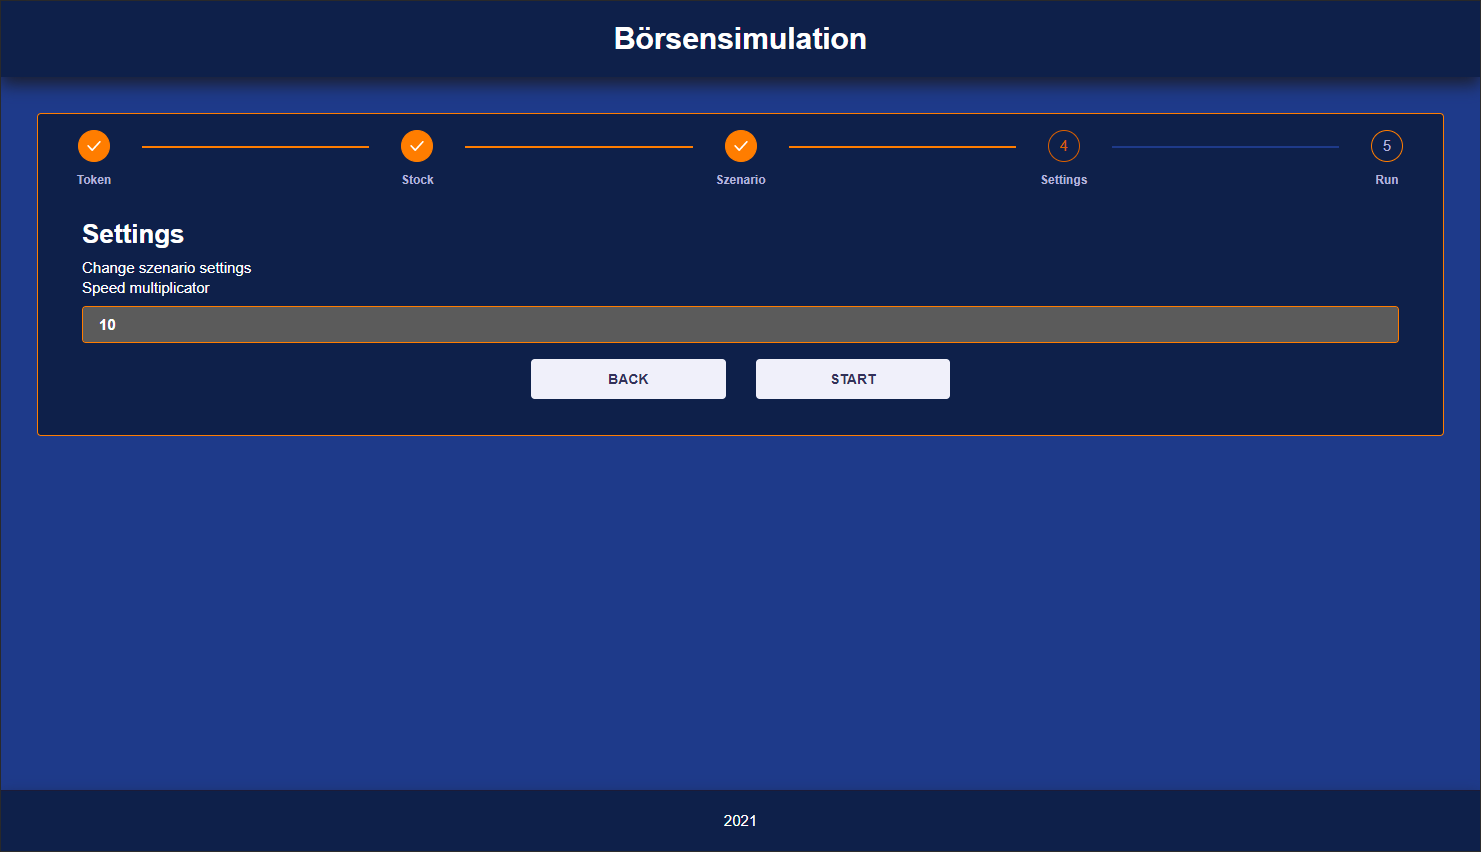
\includegraphics[width=\textwidth]{img/Settings.png}
	\centering
	\caption{Auswahl der Settings}
	\label{fig:settings}
\end{figure}

Nun läuft das Szenario. Der Balken mit der Inschrift Running, zeigt den Fortschritt des ausgewählten Szenarios. Über den Stop Button kann dies jederzeit wieder gestoppt werden. Die Wirkung des Szenarios und das Testen von eigenen Strategien kann nun mit den durch die Broker und die Börse bereitgestellten Daten und Tools bewertet werden. 
\begin{figure}[ht]
	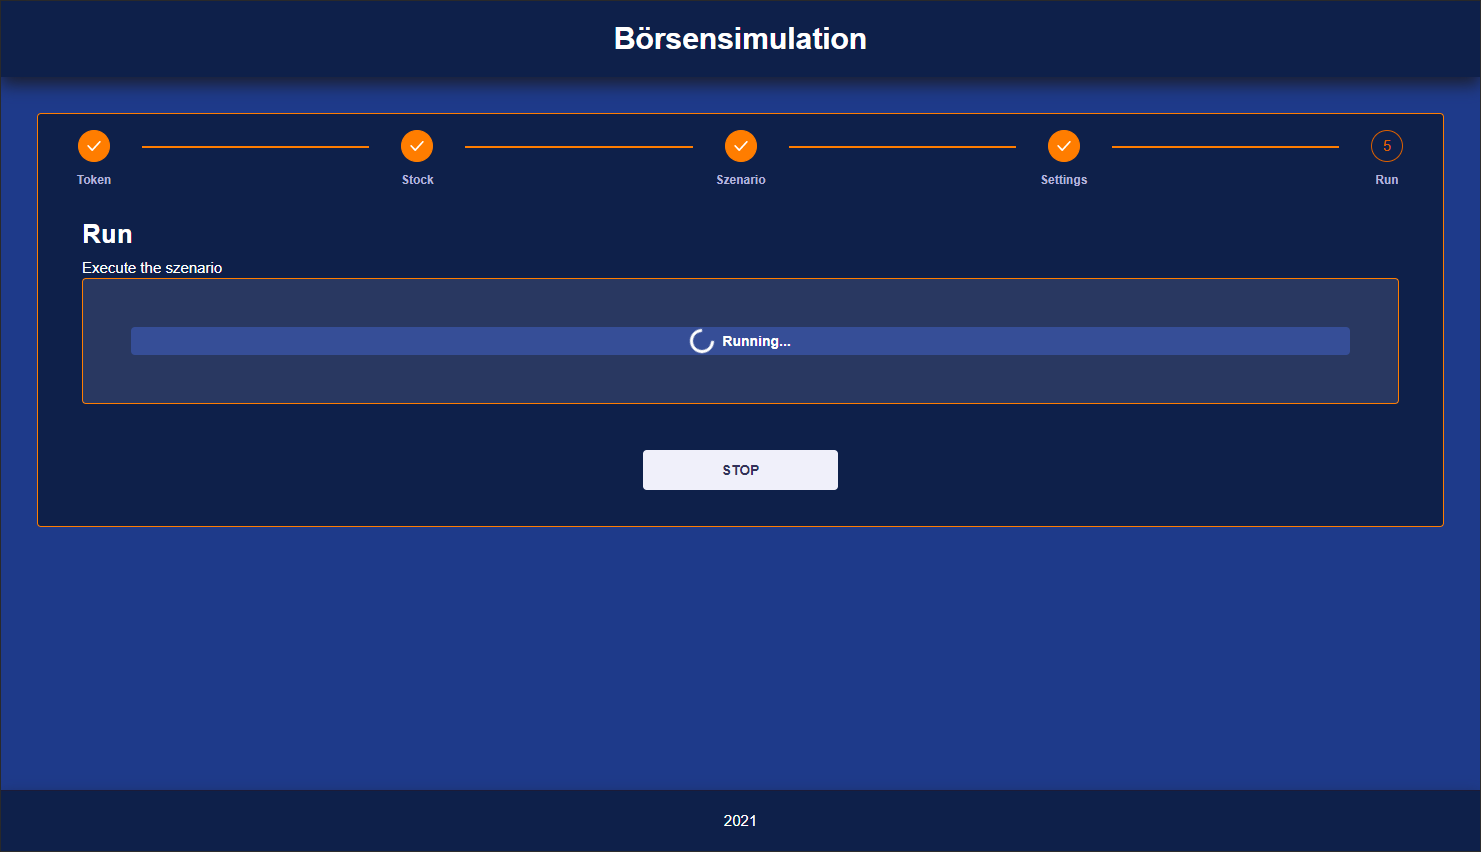
\includegraphics[width=\textwidth]{img/Run.png}
	\centering
	\caption{Laufendes Szenario}
	\label{fig:run}
\end{figure}